%% GENERATED by tools/from_docs.py from stepss-docs. Do not edit by hand:
%% edit the page named below in stepss-docs and regenerate.
%% source: stepss-docs/src/content/docs/test-systems/5bus.md

\chapter{The 5-bus tutorial system}\label{doc:ts-5bus}

The 5-bus test system is a minimal power system suitable for learning the STEPSS tools and experimenting with dynamic simulation concepts. It is small enough to trace every computation step while still demonstrating the full simulation workflow, and runs in either edition: in Python as shown below, or in \hyperref[doc:gui-first-run]{STEPSS GUI}, which ships it as a bundled example.

\textbf{Repository:} \href{https://github.com/SPS-L/stepss-5-bus-test-system}{SPS-L/stepss-5-bus-test-system}

\section{One-line Diagram}\label{ts-5bus:one-line-diagram}

\begin{figure}[htbp]
\centering
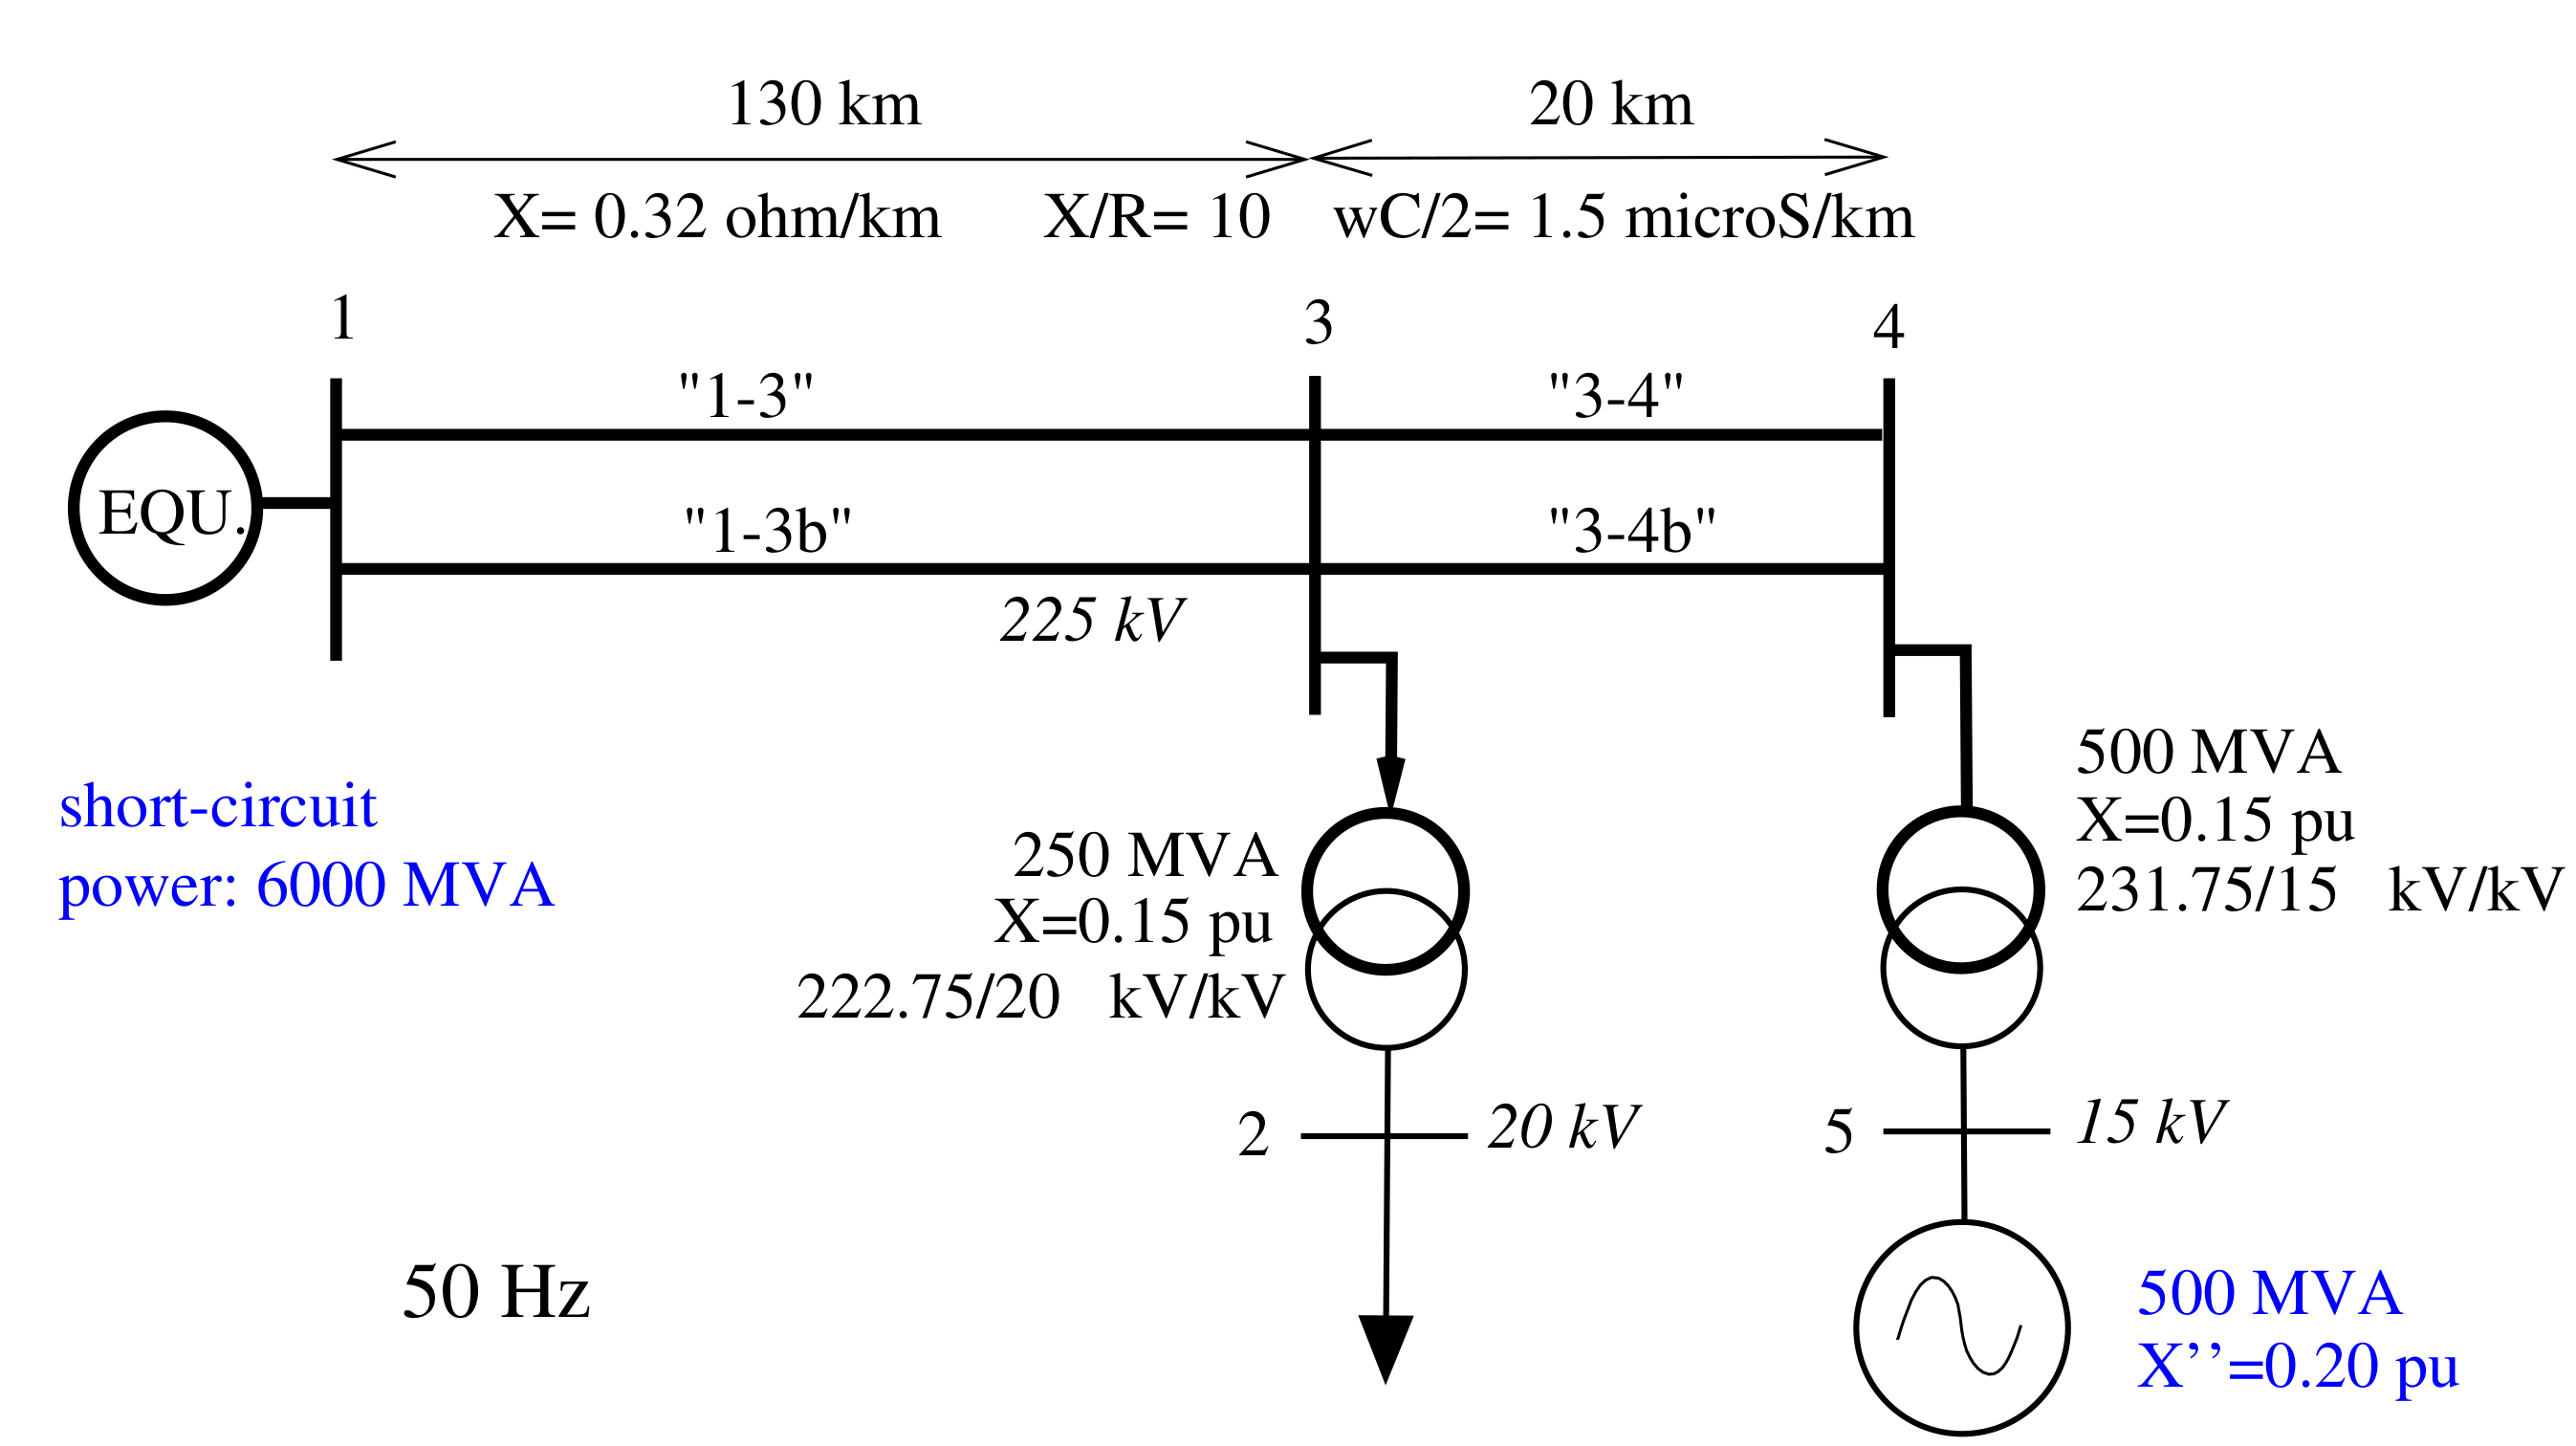
\includegraphics[width=0.70\linewidth]{figures/5bus_oneline}
\caption{One-line diagram of the 5-bus test system}
\end{figure}

\begin{center}\rule{0.5\linewidth}{0.5pt}\end{center}

\section{Quick Start}\label{ts-5bus:quick-start}

\begin{Verbatim}
import stepss
import os

# Configure the test case
case = stepss.cfg()
case.addData('dyn.dat')           # dynamic model data
case.addData('lf1solv.dat')       # power-flow solution
case.addData('solveroptions.dat') # solver settings
case.addDst('nothing.dst')        # no pre-defined disturbances
case.addObs('obs.dat')            # observables to record
case.addTrj('output.trj')        # trajectory output file

# Remove stale output files from previous runs
for f in os.listdir('.'):
    if f.endswith('.trj') or f.endswith('.trace'):
        os.remove(f)

# Run simulation with exciter setpoint change
ram = stepss.sim()
ram.execSim(case, 0.0)
ram.addDisturb(1.0, 'CHGPRM EXC G Vo 0.05 2')  # +0.05 pu step on Vo at t=1 s
ram.contSim(60.0)
ram.endSim()

# Extract and plot results
ext = stepss.extractor(case.getTrj())
ext.getSync('G').P.plot()     # active power
ext.getSync('G').Q.plot()     # reactive power
\end{Verbatim}

\begin{center}\rule{0.5\linewidth}{0.5pt}\end{center}

\section{Download}\label{ts-5bus:download}

The test system files are available in the \href{https://github.com/SPS-L/stepss-5-bus-test-system}{stepss-5-bus-test-system repository}.

\section{See Also}\label{ts-5bus:see-also}

\begin{itemize}
\tightlist
\item
  \hyperref[doc:ts-index]{Test Systems}, the other benchmark networks
\item
  \hyperref[doc:py-examples]{Python API Examples}, Complete Python simulation workflow with this test system
\end{itemize}
